\documentclass[11pt]{article}
\usepackage[utf8]{inputenc}

\title{Generative Adversarial Networks}
\author{Jacob Smith}
\date{December 5, 2017}

\usepackage{natbib}
\usepackage{graphicx}
\usepackage[options ]{algorithm2e}
\usepackage{parskip}

\graphicspath{{./img/}}

\begin{document}
\maketitle

\begin{abstract}
    Within the past decade, deep generative networks have often fallen short, especially when compared to deep discriminative models. However, since their inception in 2014, generative adversarial networks (GANs) have proved themselves as promising a research avenues for deep generative models. These networks now offer encouraging results for both unsupervised learning and generative models. The goal of this research paper is to present an overview of generative adversarial networks. Specifically, we will examine the motivation and challenges associated with GANs, their training process, architecture variations and some applications that are currently being explored.
\end{abstract}



\section{Introduction}
Deep learning has made astounding progress within the past decade. Discriminative models have already surpassed the abilities of humans to recognize patterns within certain domains \citep{2014arXiv1404.7828S}. These successes can attributed to vast, high dimension datasets in conjunction with large neural networks using linear activation functions, dropout regularization techniques and backpropagation to update the parameters \citep{2014arXiv1406.2661G}. However, deep learning possesses much more ambitious goals within the realm of unsupervised learning. As humans, we are able to understand the world around us with tremendous precision. It is easy to underestimate the complexity of the data we process to accomplish this feat. Although progress within the machine learning field is rapidly advancing, computers still have limited understanding of the data the process. Generative models, especially deep generative models such as GANs, offer promising results towards this formidable challenge \citep{genmodelingopenai}.

\subsection{Generative Modeling}
Generative models learn the joint probability distribution $p(x,y)$ of an input $x$ and label $y$ whereas discriminative models directly learn the conditional probability $p(y|x)$. An example of this process can be seen in figure \ref{fig:pdf}. Generative models may be used as classifiers using Bayes rules to calculate the conditional probability $p(x,y)$ which can then be used to make predictions \citep{NIPS2001_2020}. Although, generative models offer several other applications due to their knowledge of the underlying data distribution. Depending on the model, knowledge of the probability distribution can be created both explicitly and implicitly \citep{Goodfellow-et-al-2016}. Those which do not directly model a probability distribution offer mechanisms which require implicit knowledge of the underlying distribution, such as geminating a sample from that distribution \citep{Goodfellow-et-al-2016}.

\begin{figure}
\centering
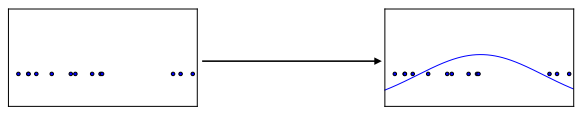
\includegraphics[scale=0.7]{pdf}
\caption{The process density estimation of one-dimensional data and a Gaussian distribution \citep{2017arXiv170100160G}. Generative models take a dataset $D$, sourced from a distribution $p_{data}$ and create an estimate of the distribution $p_{model}$.}
\label{fig:pdf}
\end{figure}

The process of training a generative model is very similar to a discriminative model. Using large amounts of data collected from a specific domain, we train the generative model to generate data from that domain. As these models typically have fewer parameters than that the number of data samples, they are forced to internalize some representation of the data \citep{genmodelingopenai}. This process within the context of GANs is elaborated in section \ref{sed:latentspace}. Unlike supervised training, there exists no single desired output. The problem becomes defining a cost function which forces the generative model to produce data more like that of the target domain \citep{genmodelingopenai}.

\subsection{Generative Adversarial Networks}
Generative adversarial networks (GANs), first introduced in 2014 by Goodfellow \textit{et al.}, offer a new framework for estimating generative models with use of an adversarial process \citep{2014arXiv1406.2661G}. These models offer a clever approach to solving the aforementioned problem of explicitly defining a cost function. Rather than training a single model, a discriminator is introduced. These two networks are pitted against each other in a minimax, zero-sum game. The generative model $G$ attempts to produce data that resembles that of the training set while the discriminative model $D$ attempts to discriminate between a real and generated (fake) sample. To train this network, $G$ attempts to maximize the error rate of $D$ whereas $D$ attempts to minimize it. The goal of the GAN algorithm is to reduce the distance between the data and generated probability distributions. Backpropagation is used to update the parameters and to train each model. In the ideal case, $D$ is unable to distinguish the generated samples from the real samples and produces an error rate of $\frac{1}{2}$ \citep{2014arXiv1406.2661G}.

The adversarial process is often analogized to a counterfeiter trying to fool a detective \citep{2014arXiv1406.2661G}. The detective will receive both real and counterfeited money and will try and distinguish between the two. This leads to a competitive scenario where both parties gradually improve their abilities until the counterfeits are indistinguishable from the true currency.

\subsection{Motivations}
There exists several compelling reasons for studying generative modeling, especially GANs \citep{2017arXiv170100160G}. Generative models are extremely useful when your goal is understand the underlying data generating distribution. The ability to learn the joint probability distribution of high dimensional data is relevant to both applied math and engineering \citep{2017arXiv170100160G}. Furthermore, GAN promise many real world applications. Several of these opportunities are expanded upon in section \ref{sec:applications}.

\subsection{Related Work}
Until the advent of GANs, most deep generative models provided a parametric specification of an probability distribution function \citep{2014arXiv1406.2661G}. These models could be trained using maximum likelihood estimation which often required gradient estimation. The most successful of these models is the deep Boltzmann machine \citep{2014arXiv1406.2661G}. The difficulties associated with gradient estimation motivated the development of \textit{generative machines}, models which implicitly represent the joint probability distribution by generating samples from that distribution rather than explicitly rendering a probability distribution.

Deep generative stochastic networks are an example of a generative machine. This model, developed by Bengio \textit{et al.} in 2013 \citep{2013arXiv1306.1091B}, was able to use backpropagation during training; however, still made use Markov chains which introduced instability problems. GANs extend the ideas presented within generative stochastic networks by eliminating the use of Markov chains \citep{2014arXiv1406.2661G}.



\section{Background}
The goal of the GAN training process is to determine the discriminator and generator parameters such that the classifier error is minimized and maximized respectively \citep{2017arXiv171007035C}. GANs may use any differentiable functions for their underlying implementation; however, optimal results are typically achieved when neural networks are used \citep{2014arXiv1406.2661G}. We first define a vector $z$ which is sampled from a prior noise distribution $z~p_z(z)$. This vector becomes the argument of the generator $G(z;\theta_g)$ where $G$ is a differentiable function and $\theta_g$ are its parameters. Another differentiable function $D(x;\theta_d)$ is defined for the discriminator. This function takes as input a vector $x$ from either the output of $G$ or a sample from the training set and is parametrized by $\theta_d$. The output of the discriminator is a scalar number which represents the probability that the sample $x$ was derived from the training data. In this situation, there exists a minimax game, a scenario derived from game theory, where $D$ attempts to maximize the probability of assigning a correct label and $G$ attempts to minimize $\log(1-D(G(z)))$. The value function $V(D,G)$ becomes:

$$\min_{G}\max_{D}V(D, G) = \mathbb{E}_{x\sim p_{data}(x)}\Big[\log(D(x))\Big] + \mathbb{E}_{z\sim p_z(z)}\Big[\log(1-D(G(z)))\Big]$$

\subsection{Cost Functions}
For training, any variant of gradient descent may be used \citep{2017arXiv170100160G}. The first part of the training step involves updating $\theta_D$ while attempting to minimize the discriminator cost function $J_D$. The next part involves updating $\theta_G$ while attempting to minimize the generator cost function $J_G$. There exist several variations of the cost function that may be used for training purposes; however, the discriminator cost has remained the same:

$$J^{(D)}(\theta_D,\theta\G) = -\frac{1}{2}\mathbb{E}_{x\sim p_{data}(x)}\Big[\log(D(x))\Big] - \frac{1}{2}\mathbb{E}_{z\sim p_{z}(z)}\Big[\log(1-D(G(z)))\Big]$$

This is a standard cross entropy cost function that is trained on two minibatches, one from the dataset and one from the generator. For this to become a zero-sum game, the cost function of the generator is simply the negation of the discriminator:

$$J^{(G)}(\theta_D,\theta\G) = -J_d(\theta_D,\theta\G)$$

This version of the generator loss function is particularly useful for theoretical analysis as shown in the original GAN paper \citep{2014arXiv1406.2661G}. Goodfellow demonstrated that the learning within the minimax game is identical to minimizing the Jensen-Shannon divergence and that each player will eventually converge if both players are able to directly update the function space as oppose to the parameters within the network \citep{2017arXiv170100160G}. However, in this minimax version, the loss function of the generator suffers from a vanishing gradient when the discriminator confidently rejects the generated data. The solution proposed by Goodfellow is to train the generator to maximize $log(D(G(z)))$ rather than minimize $log(1-D(G(z)))$ \citep{2014arXiv1406.2661G}. This function is heuristically motivated as to provide strong gradients when either the generator or discriminator is not functioning optimally. In this version, the generator attempts to maximize the log probability of a misclassification whereas the minimax version attempts to minimize the log probability of the discriminator being correct:

$$J^{(G)}(\theta_D,\theta\G) = -\frac{1}{2}\mathbb{E}_{z\sim p_{z}(z)}\Big[\log(D(G(z)))\Big]$$

A maximum likelihood cost is another option for training GANs \citep{2017arXiv170100160G}. It can be shown that that this cost function minimizes the Kullback-Leibler divergence between $p_{data}$ and $p_{model}$ instead of the Jensen-Shannon divergence. This cost estimator is useful as it allows for comparison with other generative models; however, it behaves similarly to the minimax cost function as seen in figure \ref{fig:CostFunc}.

$$J^{(G)}(\theta_D,\theta\G) = -\frac{1}{2}\mathbb{E}_{z\sim p_{z}(z)}\Big[\exp(\sigma^{-1}(D(G(z))))\Big]$$

\begin{figure}
\centering
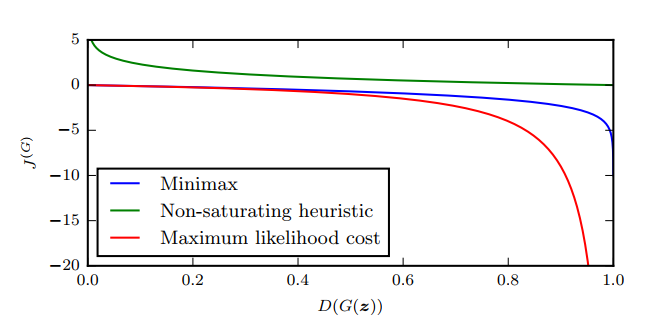
\includegraphics[scale=0.5]{costfunc}
\caption{A comparison of the generator cost function for generative adversarial networks. When $D(G(z))$ is close to $0$, the gradient is saturated for both the minimax and maximum likelihood cost functions. This situation occurs when the discriminator $D$ confidently rejects the generated sample $G(z)$. Therefore, the non-saturated heuristic cost function is the only one which works well in practice. Furthermore, the maximum likelihood cost function may produce high variance due to the rapid decrease of $J^{(G)}$ as $D(G(z))$ nears $1$. Image retrieved from Goodfellow's NIPs tutorial \citep{2017arXiv170100160G}.}
\label{fig:CostFunc}
\end{figure}

\subsection{Algorithm}
This following algorithm presents initial training algorithm used by Goodfellow \textit{et al.} when GANs were introduced in 2014 \citep{2014arXiv1406.2661G}. The first step in the algorithm is to optimize the discriminator $D$. Many researchers initially held the belief that it would be optimal to train $D$ more steps than the generator; however, this is still a controversial topic among researchers \citep{2017arXiv170100160G}. It is Goodfellow's opinion that each model should be trained simultaneously \citep{2017arXiv170100160G}.

\begin{algorithm}[H]
  \SetAlgoLined
  \Input{$n$: The number of training iterations} \linebreak
  \Input{$k$: The number of discriminator iterations} \linebreak
  \For{training iteration in n} {
    \For{discriminator iteration in k} {
      sample $m$ vectors $\{z^{(1)},...,z^{(m)}\}$ from distribution $p_z(z)$\;
      sample $m$ vectors $\{x^{(1)},...,x^{(m)}\}$ from the training samples\;
      update the discriminator using its stochastic gradient
      $$\nabla_{\theta_d}\frac{1}{m}\sum_{i=1}^{m}[\log(D(x^{(i)}))+\log(1-D(G(z^{(i)})))]$$
    }
    sample $m$ vectors $\{z^{(1)},...,z^{(m)}\}$ from distribution $p_z(z)$\;
    update the generator using its stochastic gradient\;
    $$\nabla_{\theta_g}\frac{1}{m}\sum_{i=1}^{m}[\log(1-D(G(z^{(i)})))]$$
  }
  \caption{The initial generative adversarial network algorithm developed by Goodfellow \textit{et al.} in 2014 \citep{2014arXiv1406.2661G}. Multiple variations of this algorithm have since been produced. One of the benefits of adversarial networks is that they may be updated using back propagation.}
\end{algorithm}



\section{Issues}
There exist several issues that characterize generative adversarial networks. Some are related design of GANs or their underlying network implementations. These issues lay at the forefront of GAN research.

\subsection{Instability} \label{sec:instability}
Generative adversarial networks are often characterized by their instability \citep{2017arXiv170100160G}. The training process makes use of gradient descent which does not guarantee convergence to the Nash equilibrium, the game theory equilibrium that involves two competing players. This training process for GANs is different than network optimization which is common in discriminative models. When either the generator or discriminator trains, even if that specific network improves, the other may regress. This sometimes leads to the scenario where each network repeatedly undo's the other's progress. This problem is not specific to GANs, but to any zero-sum game situations \citep{2017arXiv170100160G}.

Goodfellow has demonstrated that convergence is guaranteed if updates are made directly to the function space; however, this is obviously not what occurs. During training, we only ever update the parameter space \citep{2014arXiv1406.2661G}. As of yet, no theoretical justifications have been found that guarantee convergence or non-convergence when updates are only made to the parameters \citep{2017arXiv170100160G}. In practice, adversarial networks often oscillate between different kinds of samples without converging to an equilibrium in a phenomenon called mode collapse.

\subsection{Mode Collapse}
Mode collapse occurs when the generator collapses several different latent space vectors $z$ to the same outputs. This problem can be visualized in figure \ref{fig:modecollapse}. Full mode collapse is rare; however, partial mode collapse often occurs and varies by intensity \citep{2017arXiv170100160G}. For example, the generator may create several images that contain the same object at different perspectives, but generated with dissimilar vectors. This occurs when the capacity of the generator is superior to that of the discriminator. Backpropagation does not necessarily follow the minimax game mentioned earlier and may behave like the maximin version:

$$G^* = \max_{D}\min_{G}V(F, D)$$

When this occurs, the generator attempts to map every $z$ vector to the one $x$ variable the discriminator is most likely to guess is real. When training, one can only hope the behavior of gradient descent resembles the minimax version. It is often speculated that the root cause of the issue is the particular divergence measure used \citep{2017arXiv170100160G}. Specifically, it is often asserted that mode collapse is caused by the use of Jensen-Shannon divergence; however, the use of Kullback-Leibler divergence has be shown to worsen the problem \citep{2017arXiv170100160G}. As mode collapse is currently an unavoidable reality for GANs, their applications are limited to situations where it is acceptable to generate only a small number of distinct outputs \citep{2017arXiv170100160G}. However, recent progress has been made to reduce this problem. A potential solution is discussed in section \ref{sec:minidisc}.

\begin{figure}
\centering
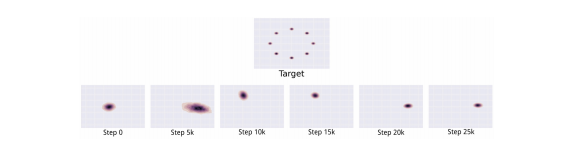
\includegraphics[scale=0.8]{modecollapse}
\caption{An example of mode collapse as demonstrated by Metz \textit{et al.} \citep{2016arXiv161102163M}. The generated samples cluster around only one of the modes and do not spread out as they should. Throughout the training process, this cycle continues does not reach an equilibrium.}
\label{fig:modecollapse}
\end{figure}

\subsection{Image Quality}
When generating images, problems often arise due to the generators difficulties with perspective, counting and structure \citep{2017arXiv170100160G}. For example, an generated animal may  have a 2D structure, misplaced limbs or too many of a specific body part. These issues arise due to the underlying model architecture, typically convolutional neural networks, and are not a direct problem of the adversarial network \citep{2017arXiv170100160G}. Furthermore, generated image resolution has remained relatively low; however, recent improvements outlined in section \ref{sec:proggans} show improvements with regard to resolution.

\subsection{Evaluation}
The evaluation procedure for generative adversarial networks remains an open debate as there exist no clear quantitative measurement to evaluate the models \citep{2017arXiv170100160G}. For example, models with high likelihood may produce unrealistic samples and models with low likelihood may produce realistic samples \citep{2017arXiv170100160G}. Several variations of the GANs examine the tradeoffs of divergence measures other than the original Kullback-Leibler divergence \citep{2015arXiv151101844T}. It has been shown that different metrics lead to different tradeoffs and different evaluations favor different models \citep{2015arXiv151101844T}. Therefore, it is important to asses one's model within the context of the whole application \citep{2015arXiv151101844T}.

\subsection{Discrete Data}
GANs assume a model implementation that is differentiable due to it's use of back propagation. Therefore, this restricts their ability to generate discrete data. Goodfellow proposes several solutions such as algorithm modifications, discretization of outputs or the use of concrete distributions or Gumbel-softmax \citep{2017arXiv170100160G}.



\section{Training Improvements}
A substantial amount of research has been conducted within the past three years with regards to improving GAN training procedures. A paper released by Salimans \textit{et al.} while at OpenAI outlines several techniques that can be applied to improve the GAN training process \citep{2016arXiv160603498S}. As mentioned in section \ref{sec:instability}, the optimal solution for GANs is the convergence to the Nash equilibrium of the minimax game; however, gradient descent only attempts to minimize the cost function and not to find the Nash equilibrium. The following techniques introduced in the paper address the instability of GANs and attempt to increase the probability of convergence.

\subsection{Feature Matching}
Feature matching involves the definition of a new cost function for GANs so that the generator does not overtrain on the current discriminator \citep{2016arXiv160603498S}. Instead of optimizing on the output of the discriminator, the new objective requires the generator to minimize the difference between the expected value of some intermediate layer. The objective function can be described as $\Big|\Big|\mathbb{E}_{x\sim p_{data}(x)}\Big[f(x)\Big] - \mathbb{E}_{z\sim p_{z}(z)}\Big[f(G(z))\Big]\Big|\Big|_2^2$ where $f(x)$ is the output of the activation function of some layer of the discriminator. Experimental evidence gathered has demonstrated the usefulness of this technique, especially when the training process becomes instable \citep{2016arXiv160603498S}. Furthermore, feature matching is useful for semi-supervised GAN applications as will later be described in section \ref{sec:semisupervised}.

\subsection{Minibatch Discrimination} \label{sec:minidisc}
Minibatch discrimination attempts to minimize the issues caused by mode collapse. This problem occurs as the discriminator processes each value $x$ independently of each other value. The gradients of discriminator will all point in the same direction, thus leading to mode collapse. This technique involves the use of a minibatch in place of a single value to allow to discriminator to examine multiple data examples at one time. The discriminator is then able to examine the distance between each sample in conjunction with the samples themselves and look for abnormal minibatch distributions. Successful applications of this technique allow for visually appealing images to be generated much quicker than by previous training techniques \citep{2016arXiv160603498S}. Preliminary results also show great reduction of mode collapse issues \citep{2017arXiv170100160G}.

\subsection{Historical Averaging}
Historical averaging introduces an extra term for each player's cost function such that they are penalized when choosing new parameters that differ from the historical mean value \citep{2016arXiv160603498S}. The new term becomes $||\theta - \frac{1}{t}\sum_{i=1}^{t}\theta[i]||^2$ where $t$ is the total number of iterations performed and $\theta[i]$ is the value of the parameters at iteration $i$. This technique has been demonstrated to help low dimensionality games reach an equilibrium where normal gradient descent has failed \citep{2016arXiv160603498S}.

\subsection{Label Smoothing}
Label smoothing was a technique first introduced in the 1980s which involves replacing the 0 and 1 targets with \textit{smoother} values such as 0.1 and 0.9 respectively \citep{2016arXiv160603498S}. This technique is used to improve the networks resistance to adversarial examples. Specifically, it is recommended one use only one-sided label smoothing by using 0.9 label instead of 1 for the real data label. If one alters the label for fake data, problems may arise when $p_{data}(x)$ nears $0$ and $p_{model}(x)$ becomes large for some sample $x$ \citep{2016arXiv160603498S}.

\subsection{Virtual Batch Normalization}
Batch normalization is a technique that was first introduced in 2014 which involves applying normalization for each training minibatch \citep{2015arXiv150203167I}. It allows for much higher learning rates, a more stable training process and a reduction of problems associated with parameter initialization \citep{2015arXiv150203167I}. This normalization technique has proved useful for GAN training; however, it often causes a dependence relationship between the samples of the minibatch \citep{2016arXiv160603498S}. A new technique called virtual batch normalization (VBN) was developed where a reference batch of samples is randomly chosen at the start of the training process and used throughout to normalize each training sample. However, this technique is computationally expensive as it requires forwarding two minibatches and it is recommended to only use VBN for the generator \citep{2016arXiv160603498S}.



\section{Architecture Variations}
Research within the field of deep generative modeling has increased exponentially since the debut of generative adversarial networks in 2014. Significant improvements are being made with respect to image quality and training stability. Hundreds of papers have been released since 2014 (see figure \ref{fig:CumulativeNumberofGANPapersbyMonth}) which propose numerous architectural variations.

\begin{figure}
\centering
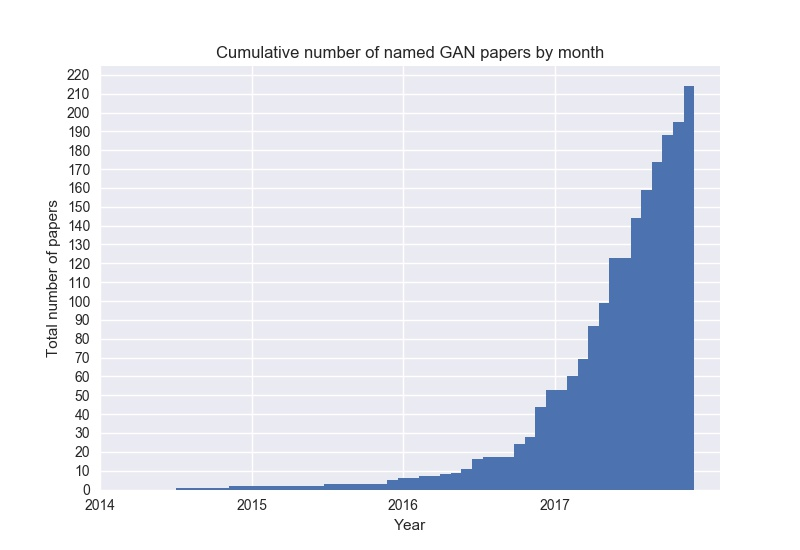
\includegraphics[scale=0.43]{cumulative_gans}
\caption{The cumulative amount of papers written about generative adversarial networks. The graph shows the exponential growth of GANs within the past three years. Image maintained by Avinash Hindipur \citep{November2017GANZoo}.}
\label{fig:CumulativeNumberofGANPapersbyMonth}
\end{figure}

\subsection{Fully Connected GANs}
The first generative adversarial network paper by Goodfellow \textit{et al.} made use of relatively simple fully connected neural networks for the generator and discriminator models \citep{2017arXiv171007035C}. These are networks where each neuron in one layer is connected to every neuron in the following layer. This design is able to generate simple images and useful for proof of concept; however, several other architectures have overtaken this implementation \citep{2017arXiv171007035C}.

\subsection{Convolutional GANs}
Although convolutional neural networks (CNNs) seem well suited for the image generation tasks associated with GANs, difficulties associated with training initially constrained the use of convolutional models for both the discriminator and generator \citep{2017arXiv171007035C}. When implementing CNNs within a GAN, one is often unable to train the discriminator and generator to the same level of capacity and representational power when compared to supervised CNN models \citep{2017arXiv171007035C}. One solution proposed by Denton \textit{et al.} made use of Laplacian pyramids (LAPGAN) to address this problem \citep{2015arXiv150605751D}. A Laplacian pyramid is a type of multi-scale signal representation which repeatedly smooths and downsamples an image to form a sort of pyramid of images. At each layer of the pyramid, a conditional convolutional GAN (see section \ref{sec:condgan}) is trained given the generator output of the above layer.

Another solution to this problem was proposed by Radford \textit{et al.} made alterations to conventional deep convolutional network architecture \citep{2015arXiv151106434R}. Max pooling was replaced with strided layers within the discriminator and fractionally-strided layers within the generator. Furthermore, LeakyReLUs are used for all layers of the discriminator in place of the standard ReLU non-linearity function. The fractionally strided layers within the generator replicate the benefits of the progressive upscaling within the Laplacian pyramid \citep{2017arXiv171007035C}. The strided layers allow the GAN to learn both the down-sampling and up-sampling operators during training \citep{2017arXiv171007035C}. This architecture, called DCGAN, has become the base model for most GANs today \citep{2017arXiv170100160G}.

\subsection{Conditional GANs} \label{sec:condgan}
Initially proposed by Goodfellow as a straightforward extension of the first GAN architecture \citep{2014arXiv1406.2661G}, Mirza \textit{et al.} successfully implemented a conditional generative model in late 2014 \citep{2014arXiv1411.1784M}. A generative model differs from a conventional models as an additional parameter $c$ is given to both the generator $G(z|c)$ and discriminator $D(x|c)$ to condition the GAN. The new objective function of a conditional GAN becomes:

$$\min_{G}\max_{D}V(D, G) = \mathbb{E}_{x\sim p_{data}(x)}\Big[\log(D(x|c))\Big] + \mathbb{E}_{z\sim p_z(z)}\Big[\log(1-D(G(z|c)))\Big]$$

These architectures are better suited for multi-modal output as they are able to provide better data representations \citep{2017arXiv171007035C}. By conditioning the GAN, it is possible to control the data generation process. This additional input may be class label or other items such as text or an image. In section \ref{sec:img2img}, we will see how conditional GANs are applied to image translation tasks.

\subsection{Inference GANs} \label{sec:inferencegan}
The first GAN architectures lacked the ability to map an sample $x$ to its associated latent vector $z$. The ability to do this is often referred to as having an \textit{inference mechanism} \citep{2017arXiv171007035C}. In 2016, two new architectures were independently proposed which introduced this mechanism by adding an inference network \citep{2016arXiv160509782D, 2016arXiv160600704D}. This new architecture involves two generative models, a decoder and encoder, which work together to fool the discriminator. The discriminator is now trained with a sample $x$ and latent space vector $z$ and has to decide if the pair is a real sample and its encoding or generated image and its associated latent space input. This architecture allows the encode to learn the mapping of $x$ to $z$. Furthermore, it generates a set of continuous variables. That is, if the vector $z$ is of length $n$, then $n$ means and $n$ variances will be generated. This allows for a probability distribution for each value of $z$. However, the reconstructed images still remain of poor quality \citep{2017arXiv171007035C}.

\subsection{Progressive GANs} \label{sec:proggans}
Progressive GANs do not offer an architecture variation but a new training methodology for training GANs. Introduced in October 2017 by Karras \textit{et al.} \citep{2017arXiv171010196K}, these networks incrementally increase the number of convolutions within both the generator and discriminator. Each new convolution is only added after the previous GAN converges. This permits the generator to progressively discover the image distribution, increases the training speed and reduces training instability \citep{2017arXiv171010196K}. Combined with new normalization techniques, progressive GANs allow for much higher resolution images to be generated \citep{2017arXiv171010196K}. The experimental results offer promising new directions for GAN research and applications.

\begin{figure}
\centering
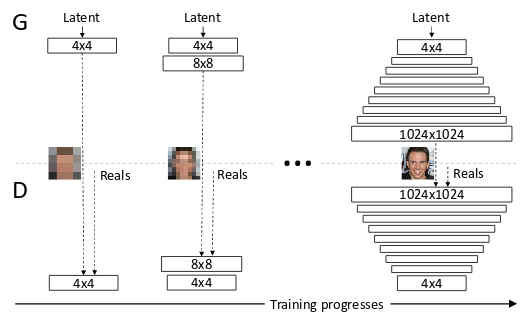
\includegraphics[scale=0.45]{progressive_growing}
\caption{The training process of progressively growing generative adversarial networks recently introduced by Karras \textit{et al.} \citep{2017arXiv171010196K}. The generator and discriminator begin at $4x4$ resolution and progressively grow generate and discriminate $1024x1024$ resolution images.}
\label{fig:ProgressiveGrowingGAN}
\end{figure}



\section{Latent Space} \label{sed:latentspace}
The generator model of a GAN must internalize a representation of the data that it is trained on. This quality is shared with variatinal autoencoders and word linguistic models such as \textit{word2vec} \citep{2017arXiv171007035C}. One interesting characteristic of the latent space is that it is typically of lower dimension than the training data \citep{2017arXiv171007035C}. This forces the model to efficiently represent the training data by extracting only useful features. As long as the effects of mode collapse are minimal, the latent space can be highly structured \citep{2017arXiv171007035C}. We often observe semantic transformations when interpolations are conducted. For example, movement of the latent vector in certain directions may alter rotation, produce colour changes or see the addition of attributes such as eyeglasses \citep{2017arXiv171007035C}.

As mentioned in section \ref{sec:inferencegan}, it is possible to train an encoder to map a sample $x$ to a latent vector $z$. This is an extremely useful feature for exploring the latent space \citep{2017arXiv171007035C}. For example, one may discover \textit{concept vectors} such as "wearing glasses" or "wearing a hat" and apply them to a vector associated with a human. An example of this process is illustrated in figure \ref{fig:conceptvector}.

\begin{figure}
\centering
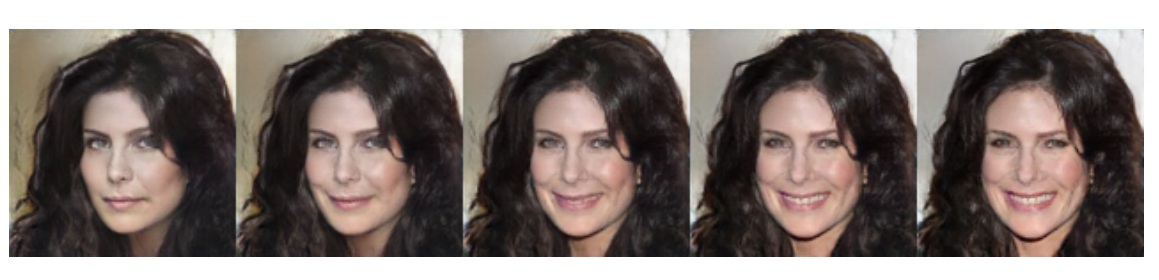
\includegraphics[scale=0.40]{smile_concept_vector}
\caption{The addition of the "smile" concept vector (far right) to a vector associated with a woman (far left). The images in-between were created through an interpolation of the two vectors. Example retrieved form Dumoulin \textit{et al.} \citep{2016arXiv160600704D}.}
\label{fig:conceptvector}
\end{figure}



\section{Applications} \label{sec:applications}
Although GANs are a relatively new invention, many different applications have already been discovered. Several of the reoccurring themes are elaborated within this section.

\subsection{Image Generation} \label{sec:img2img}
Image generation is extremely useful as many tasks intrinsically require the ability to generate realistic samples \citep{2017arXiv170100160G}. Moreover, image generator often requires the ability to model multi-modal outputs (see figure \ref{fig:multimodal}) \citep{2017arXiv170100160G}. GANs are well suited for both of these tasks. Most research conducted with respect the GANs attempts to improve the quality of synthesized images \citep{2017arXiv171007035C}. As such, several useful and fascinating image applications have already been found.

\begin{figure}
\centering
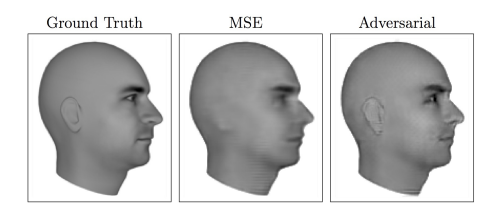
\includegraphics[scale=0.9]{multimodal}
\caption{An example of scenario where the ability to model multi-modal data is incredibly important. This figure demonstrates the process of predicting the next video frame given the previous one. A generator trained with mean squared error (middle) produces an image which averages each possible future. When using an adversarial process (right), the image produced corresponds with the most likely scenario. Example retrieved form Lotter \textit{et al.} \citep{2015arXiv151106380L}.}
\label{fig:multimodal}
\end{figure}

\subsubsection{Image Super-Resolution}
Image super-resolution is the process of generating a high resolution image from a lower resolution image by inferring details. For each lower resolution sample, there exists multiple possible correct outputs. Due to this characteristic, GANs are optimally suited for this task. The Super-Resolution GAN (SRGAN) proposed by Ledig \textit{et al.} remains similiar to other GANs; however, the discriminator is trained to distinguish real images from super-resolution images \citep{2016arXiv160904802L}. SRGANs infer photo characteristics with respect to domain of training set \citep{2017arXiv171007035C}. Therefore, it is essential to train different models for each domain of images.

\subsubsection{Image-to-Image Translation}
Image-to-image translation has made astounding progress and offers many yet undiscovered applications \citep{2017arXiv170100160G}. This process includes the translation of images from a source domain $X$ to the target domain $Y$. The translated images are then compared against images from the target domain and the generator parameters are updated as to reduce the distance between the translated and real images. An example of this operation can be visualized in figure \ref{fig:img2img}. Conditional networks are well suited for this task and there exists several different GAN architectures which take advantage of their characteristics to preform these translations \citep{2016arXiv161107004I, 2017arXiv171111585W, 2017arXiv170310593Z}. Recent work by Zhu \textit{et al.} demonstrate the feasibility of unpaired image-to-image translation by introducing a cycle consistency loss to enforce $F(G(X)) \approx X$ where $G$ is the mapper and $F$ is the inverse mapper \citep{2017arXiv170310593Z}. Furthermore, research released in November 2017 by Wang \textit{et al.} further improve the general quality of synthesized images \citep{2017arXiv171111585W}. Their semantic map translations are now almost indistinguishable from real images.

\begin{figure}
\centering
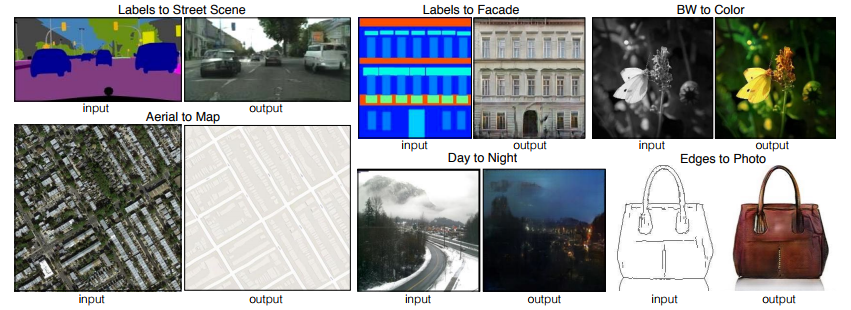
\includegraphics[scale=0.55]{img2img}
\caption{Examples of the image-to-image technique developed by Isola \textit{et al.} \citep{2016arXiv161107004I}. This technique makes use of conditional generative adversarial networks to map across image domains.}
\label{fig:img2img}
\end{figure}

\subsection{Semi-Supervised Learning} \label{sec:semisupervised}
There exist several techniques for training a classifier using a GAN. These methods all take advantage of the unsupervised aspect of GANs to implement semi-supervised learning. The ability to use GAN for unsupervised learning also offers a quantitative method to rank different GAN models.

One method involves the use of transfer learning. After the GAN training process has completed, the discriminator may be used within classification tasks as a feature extractor. A new machine learning model, such as a support vector machine (SVM), is trained on the extracted features of some layer $l$ of the discriminator. Another transfer learning approach makes use of the inference GANs mentioned in section \ref{sec:inferencegan}. Similar to the previous technique, a new machine learning model is trained on the last three hidden layers of the of the encoder. These methods have both received state-of-the-art classification results \citep{2017arXiv171007035C}.

Another general approach to semi-supervised learning involves the transformation of the discriminator into a classifier. Given that there are $k$ different labels, the new classifier will have $k + 1$ classes where the $k + 1$ class is associated with a fake image. When a real image is given to the discriminator, it attempts to classify the sample as one of the $k$ classes; however, when a generated or unlabeled image is given, the probabilities of the k classes are summed together to represent the probability of the image being real. In this situation, the classifier reverts back to its discriminative behavior. Typical supervised models need more than $50,000$ samples whereas state of the art performance can be achieved on labeled datasets ranging from $20$ to $8,000$ samples using this technique \citep{2017arXiv170100160G}.

\subsection{Reinforcement Learning}
Modeling environments offers another promising application of GANs. This capability could potentially be used for reinforcement learning and motion planning. One possible method includes the use of generative models to predict possible futures \citep{2017arXiv170100160G}. The GAN would learn a conditional distribution over future states given the current state and a hypothetical action. An agent could make multiple queries to the generator and subsequently choose the action associated with the best possible future. This technique has already been applied by Finn and Levine in 2016 \citep{2016arXiv161000696F}. Generative models may also be used to maintain a record of past actions and visited locations to aid in future decisions \citep{2017arXiv170100160G}.



\section{Conclusion}
GANs are generative models which allow us to parametrize complicated probability distribution functions. They can be used to generate, modify and manipulate images. Furthermore, they allow for the use novel techniques within the context of reinforcement learning and unsupervised learning. Today, they are already being applied to many problems \citep{genmodelingopenai}; however, the majority of their applications have yet to be discovered. As long as the research effort continues, GANs promise exciting new avenues within the field of machine learning. 

\bibliographystyle{plain}
\bibliography{references}
\end{document}

GANs build their own representations of the data they
are trained on, and in doing so produce structured geometric
vector spaces for different domains
